\documentclass[a4paper,12pt]{report}

\usepackage{alltt, fancyvrb, url}
\usepackage{graphicx}
\usepackage[utf8]{inputenc}
\usepackage{float}
\usepackage{hyperref}

% Questo commentalo se vuoi scrivere in inglese.
% \usepackage[italian]{babel}

\usepackage[italian]{cleveref}

\title{Relazione Progetto OOP\\``Dimension Holiday''}

\author{Lorenzo Prati, Elvis Perlika\\ Emanuele Dajko, Alessandra Versari}
\date{\today}


\begin{document}

\maketitle

\tableofcontents

\chapter{Analisi}

\section{Requisiti}

Il gruppo si pone l'obbiettivo di realizzare un videogioco roguelike \textit{Dimension Holiday} vagamente ispirato a giochi famosi come \textit{Hades} oppure \textit{The Binding of Isaac}. Il giocatore controllera' un personaggio che è stato trasportato in un altro mondo dove dovrà
esplorare un dungeon e affrontare un boss per tornare alla propria
dimensione.

\subsection*{Elementi funzionali}

\begin{itemize}
	\item Per attraversare tutto il dungeon il giocatore dovrà passare da stanza in stanza,
	eliminando tutti i nemici presenti. Per farlo potrà usare la spada o lanciare
	proiettili energetici. Giocatore e nemici hanno delle vite (espresse in cuori) e se il giocatore perde tutti i cuori e' \textit{Game over} e si deve ricominciare da capo
	\item Una volta che avrà ucciso tutti i nemici della stanza corrente
	compariranno dei reward casuali (cuori, monete ecc.) e il portale che
	ti trasporterà nella prossima stanza. 
	\item Dopo un certo numero di stanze, comparirà una stanza shop
	dove sarà possibile effettuare acquisti usando le monete creando una piccola progressione
	\item Il gioco si conclude quando il giocatore sconfigge un nemico speciale chiamato \textit{Boss}
	
\end{itemize}

\subsection*{Elementi non funzionali}

\begin{itemize}
	\item Ci si pone l'obbiettivo di creare un'architettura del software modulare ed espandibile ad aggiunte future, come l'aggiunta di nuovi nemici, mappe e oggetti.
\end{itemize}


\section{Analisi e modello del dominio}
Il giocatore potra' muoversi nelle 4 direzioni su, sinsitra, giu', destra tramite i tasti, rispettivamente, W, A, S, D ed effettuare due tipi di attacchi:
\begin{itemize}
	\item \textit{meele}, ovvero ravvicinato, usando una spada e tramite il tasto sinistro del mouse
	\item dalla distanza, usando un proiettile energetico e tramite il tasto destro del mouse
\end{itemize}
Il gioco dovra' essere in grado di presentare al \texttt{giocatore} una serie di stanze dove affrontare dei \texttt{nemici}. Questi potranno avere diversi comportamenti e diverse tipologie di \texttt{attacco}. Il giocatore dovrà stare attento ad evitare gli attacchi dei nemici per non perdere cuori e allo stesso tempo non entrarci in contatto, cosa che comportera' ulteriore danno.
Saranno presenti degli \texttt{oggetti} raccoglibili (cuori, monete ecc.) che dovranno applicare degli \texttt{effetti} alle entita' con cui entrano in contatto, ad esempio l'incremento della vita oppure l'incremento della valuta posseduta dal giocatore. 
Lo shop sara' gestito \textit{in game}, nel senso che non comparirà un'interfaccia grafica che permettera' al giocatore di scegliere i potenziamenti, ma il giocatore dovra' interagire dinamicamente con degli oggetti presenti nella mappa per acquistarli.
Anche gli attacchi applicheranno degli effetti con le entita' con cui entrano in contatto, come ad esempio la perdita di cuori.
Il \texttt{mondo} di gioco (\textit{dungeon}) sara' composto di una serie di stanze. Tramite l'interazione con un oggetto portale, il giocatore sara' trasportato alla stanza successiva senza possibilità di tornare indietro. All'interno delle stanze sono presenti dei muri, che bloccano il passaggio al giocatore. Esistono tre tipi di stanze: normale, shop, boss. Nella stanza normale compariranno dei nemici, in numero e tipo variabile in base al momento della partita, nella stanza shop invece compariranno gli oggetti rappresentati i potenziamenti acquistabili, e nella stanza boss comparirà solo il nemico boss.
Le stanze normali saranno intercambiate randomicamente tra un pool prescelto di mappe create a mano, mentre le stanze shop e boss saranno uniche.

La difficoltà sara' gestita in modo tale che proseguendo nel dungeon risulti piu' difficile il gioco, ad esempio facendo comparire piu' nemici nelle stanze oppure nemici piu' forti. Questo aumento della difficoltà sara' compensato dai potenziamenti che il giocatore potra' acquistare nello shop, che comparira' dopo un numero costante di stanze normali superate. 

Una delle maggiori difficoltà consistera' nella creazione di un architettura che permetta la gestione sia di diversi tipi di nemici (zombie, shooter, boss ecc.), ognuno con un proprio comportamento, sia di diversi attacchi utilizzabili sia dal giocatore che dai nemici (proiettili, attacchi meele). Inoltre, si cerchera' di realizzare un sistema di combattimento \textit{real-time} quanto piu' possibile fluido e responsivo e un'alternanza di mappe e generazione dei nemici in modo tale da far sembrare ogni partita diversa.

Dato il monte ore previsto, si rimanda al futuro una gestione accurata delle performance del gioco.

\begin{figure}[h]
	\centering{}
	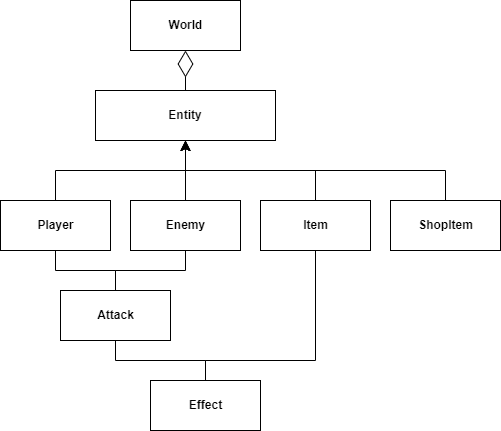
\includegraphics[width=\textwidth]{uml/img/uml_analisi_dominio.png}
	\caption{Diagramma uml concettuale rappresentante le varie entita' presenti nel dominio del gioco}
\end{figure}


\chapter{Design}



\section{Design dettagliato}


\chapter{Sviluppo}

\section{Testing automatizzato}

\section{Metodologia di lavoro}



\section{Note di sviluppo}



\chapter{Commenti finali}



\section{Autovalutazione e lavori futuri}



\section{Difficoltà incontrate e commenti per i docenti}



\appendix
\chapter{Guida utente}


\chapter{Esercitazioni di laboratorio}



\bibliographystyle{alpha}
\bibliography{13-template}

\end{document}
